\documentclass[floatfix,aps,prd,amsmath,amssymb]{revtex4}

\usepackage{hyperref}
\usepackage{epsfig}
\usepackage{color}
\usepackage{graphicx}
\usepackage{float}
\usepackage{listing} %listings
\usepackage{braket}
\usepackage{mathtools}
\usepackage[noabbrev,capitalise]{cleveref} %for \cref in CKM-Mechanism.tex 
\providecommand{\e}[1]{\ensuremath{\times 10^{#1}}} %because my scientific notation wouldn't work: Kevin

\begin{document}
\title{Title}
\author{Kevin Maguire (10318135)}
\date{\today}

\begin{abstract}
\textit{abstract}
\end{abstract}

\maketitle
\pagenumbering{roman}

%\begin{figure}[h!]
%\begin{center}
%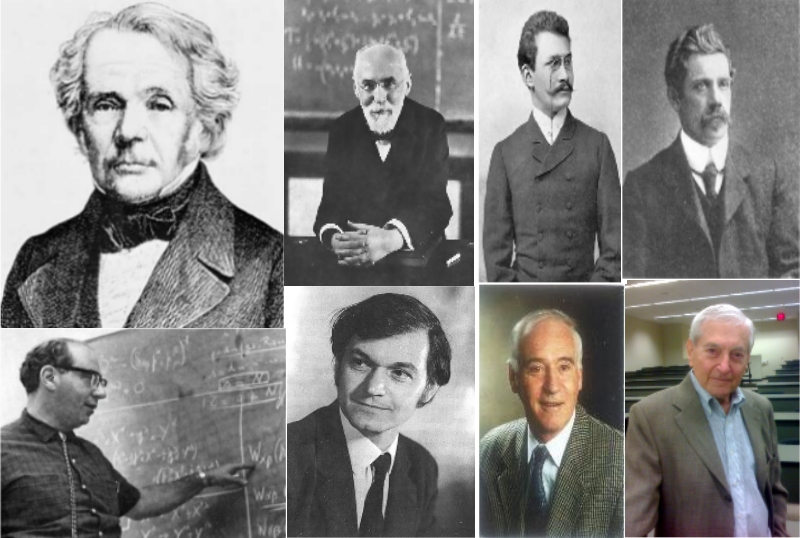
\includegraphics[scale=0.8]{figs/Cover.jpg}
%\end{center}
%\caption{\textit{}}
%\label{}
%\end{figure}

\newpage

\tableofcontents
\pagenumbering{arabic}

\newpage
 
%\input{}
 
\section{Acknowledgements}
 
\begin{thebibliography}{10}
%\bibitem{CPT}
%Hilary Greaves and Terugi Thomas - ``The CPT Theorem" - April 2012, \url{http://arxiv.org/abs/1204.4674}
\end{thebibliography}

\end{document}
